% !TEX TS-program = LuaLaTeX
\documentclass[10pt, oneside, a4paper]{article}

\usepackage[T1]{fontenc}
\usepackage{lmodern}
\usepackage{xcolor}
    \definecolor{gray} {HTML}{363636}
    \definecolor{red}  {HTML}{950009}
    \definecolor{green}{HTML}{0E610A}
    \definecolor{blue} {HTML}{020069}
    \definecolor{bglst}{HTML}{F4F4F4}
\usepackage{fontspec}
    \setsansfont{Arial}
\usepackage{amsmath}
\usepackage{titlesec}
    \titleformat*{\section}      {\color{gray}\large\bfseries\sffamily}
    \titleformat*{\subsection}   {\color{gray}\large\bfseries\sffamily}
    \titleformat*{\subsubsection}{\color{gray}\large\bfseries\sffamily}
\usepackage{geometry}
    \geometry{scale={0.75,0.85}}
\usepackage{siunitx}
    \sisetup{locale=FR}
\usepackage{graphicx}
\usepackage{caption}
    \captionsetup{labelfont={bf,sf,color=gray}}
\usepackage{pdfpages}
\usepackage{pgfplots}
	\pgfplotsset{compat=newest}
	\pgfplotsset{plot coordinates/math parser=false}
	\newlength\figureheight
	\newlength\figurewidth
\usepackage{minted}
	\setminted{linenos}
	\setminted{fontsize=\footnotesize}
	\setminted{bgcolor=bglst}
	\setminted{style=borland}
\usepackage{enumitem}

% Keep lasts
\usepackage[french]{babel}
	\frenchsetup{SmallCapsFigTabCaptions=false}
\usepackage[expansion]{microtype}
\usepackage[luatex, backref]{hyperref}
    \hypersetup{colorlinks, breaklinks, urlcolor=red,
                bookmarksopen, bookmarksnumbered}

% Generating plots is really time consuming
\usepgfplotslibrary{external}
	\tikzexternalize[prefix=figures/]

\renewcommand{\UrlFont}{\small}
\renewcommand{\arraystretch}{1.1}
\newcommand{\important}[1]{\textbf{\textsf{\color{gray}{#1}}}}
\setlength{\parskip}{8pt}

\begin{document}

\begin{titlepage}
    \centering
    
\includegraphics[width=0.5\textwidth]{images/logo-ecam.png}\par
    \vspace{1cm}

    \rule{\linewidth}{1.5pt}%
    \vspace{5mm}
    {\rm\sffamily\LARGE Techniques de transmission et traitement du signal\par}
    \vspace{3mm}
    {\sffamily\bfseries\LARGE Simulation d’une chaîne de transmission\\
    						  numérique avec Matlab\textregistered{}\par}
    \vspace{5mm}
    \rule{\linewidth}{1.5pt}%
    \vspace{1cm}

    {\large%
        \begin{minipage}[t]{0.35\linewidth}
            \centering
            Alexis~\bsc{Nootens} \\[1mm]
            \href{mailto:16139@student.ecam.be}{16139@student.ecam.be}
        \end{minipage}
        \begin{minipage}[t]{0.35\linewidth}
            \centering
            Armen~\bsc{Hagopian} \\[1mm]
            \href{mailto:14040@student.ecam.be}{14040@student.ecam.be}
        \end{minipage}
    \par}
    \vspace{1cm}

    {\large%
        ECAM Brussels             \\[1mm]
        Promenade de l'Alma 50    \\[1mm]
        1200 Woluwe-Saint-Lambert \\[1mm]
        Belgique
    \par}

    \vfill
    {\large\today\par}
\end{titlepage}

%%%%%%%%%%%%%%%%
\tableofcontents
\newpage

%%%%%%%%%%%%%%%%%%%%%%%
\section{Introduction}
L'objectif de ce projet est simuler la couche physique d'un protocol de communication, c'est-à-dire le niveau 1 du modèle OSI.
La simulation est réalisée avec le logiciel Matlab\textregistered{} édité par Mathworks\textregistered{}.
Les contraintes imposées dans la simulation sont de tenir compte de plusieurs émetteurs et receveurs pouvant communiquer en même temps.
Pour répondre à cette contrainte, la couche physique implémentée utilise le multiplexage fréquentiel.

Ce document reprend la conception du projet et les choix qui ont dû y être décidés, accompagnés de leur explication.


%%%%%%%%%%%%%%%%%%%%%%%%
\section{Implémentation}
\label{sec:implementation}
La section~\ref{sec:implementation} décrit le travail apporté dans les fichiers qui composent le projet.
Ces fichiers peuvent être consultés à l'annexe~\ref{sec:fichiers-sources}.
Ils consistent en :
\begin{description}[align=right,labelwidth=2cm,labelindent=1cm]
	\item[main.m] lance les scripts dans l'ordre logique.
	\item[parameters.m] configure paramètres de simulation.
	\item[sender.m] génère les données aléatoirement, puis sépare les canaux
		fréquentiellement.
	\item[channel.m] simule un canal de communication en atténuant et filtrant les signaux.
	\item[receiver.m] démodule les signaux reçus et tente de recomposer le signal émis.
\end{description}

\subsection{Fichier principale}
Le fichier principale, aussi nommé \og{}main\fg{} par son nom anglais, se charge de lancer la simulation dans un ordre logique.
Le fichier est consultable à l'annexe~\ref{app:main}.
Son contenu est minime, il commence par nettoyer le plan de travail de variables et figures résiduelles.
Il lance ensuite les scripts dans l'ordre parameters $\rightarrow$ sender $\rightarrow$ channel $\rightarrow$ receiver.

Une fois la simulation terminée, il affiche une figure comparant le signal dans un canal émis par sender, au signal recomposé dans ce même canal par le receveur.
La figure~\ref{fig:comparaison} présente un exemple de cette comparaison.
On peut y apercevoir que le signal recomposé est délayé par rapport au signal émis, et que son amplitude aux pics isolés est quasiment divisé par deux.
Cela est normal étant donné que l'on retrouve plus de fréquence dans un pic isolé que dans une succession à la même amplitude.
Ce pic souffrira donc plus fortement au filtrage fréquentiel.

\begin{figure}[htbp]
	\centering
	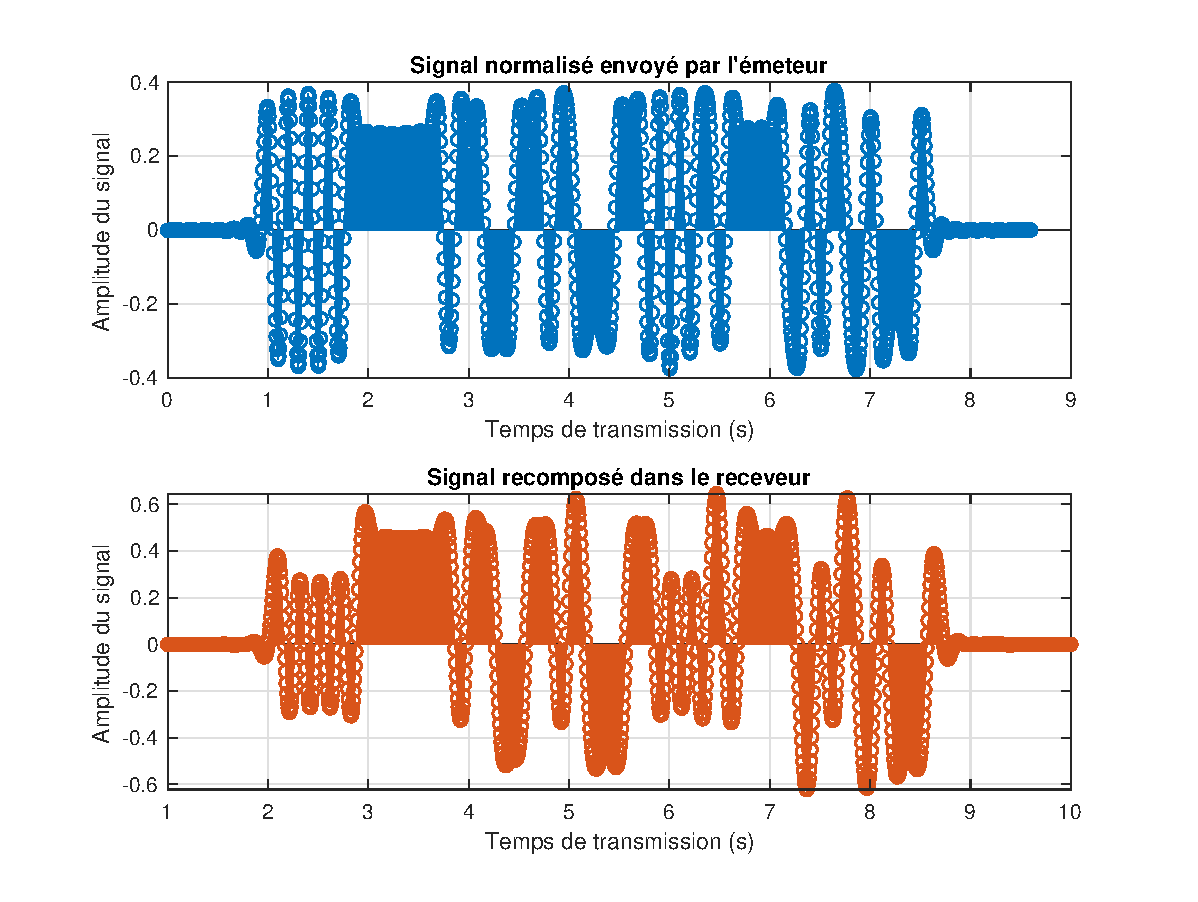
\includegraphics[height=0.45\textheight]{eps/comparaison.eps}
	\caption{Comparaison entre le signal en bande de base émis dans l'émetteur et celui
			 recomposé dans le receveur.
			 Le signal reçu est décalé d'approximativement 1 seconde par rapport au signal
			 émis.
			 Le signal reçu est également plus sévèrement atténué aux pics isolés qui
			 contiennent des plus hautes fréquences.}
	\label{fig:comparaison}
\end{figure}

\subsection{Paramètres}
Le fichier \texttt{parameters.m} offre un accès rapide et concentré aux différents paramètres influençant le simulation tel que le nombre de canaux fréquentiel disponibles, la taille du message à envoyer, ou encore la vitesse d'envoie.
Ce fichier est consultable à l'annexe~\ref{app:paremeters}.
Chaque paramètre est accompagné d'un commentaire expliquant dument son utilité.

\subsection{Émetteur}
Le fichier \texttt{emetteur.m} consultable à l'annexe~\ref{app:sender} commence la simulation à proprement dire.
Il débute par générer des bits aléatoire suivant une distribution normale.
Il rajoute une séquence de départ pour la forme uniquement, cette dernière n'est pas exploitée dans le receveur.
Les bits sont ensuite codés dans un code PAM-2 ou les 0 deviennent $-1$ et les 1 restent 1.

Afin de diviser le spectre fréquentiel pour y définir des canaux, il faut s'assurer que les messages envoyées se limite à leur bande allouée.
Pour ce faire nous utilise le filtre en cosinus surélevé qui à la merveilleuse propriété que pour un signal avec un durée de symbole $\xi$ seconde, il ne consommera que $\frac{\xi}{2}$ largeur de spectre dans le domaine fréquentiel.
C'est la meilleur efficacité spectrale atteignable mathématiquement.
Un soucis survient avec l'utilisation de ce filtre, c'est que le signal codé maintient son amplitude maximale durant un bref instant, puis chute rapidement.
Ce type de réponse n'est pas utilisable en pratique car la fréquence de capture d'échantillons dans le receveur n'est pas monotone et stable, ni même en phase.
Pour adresser ce problème, le filtre maintient son plafond durant un instant plus allongé, mais aux prix de flancs montant et descendant plus raides car la période d'expression d'un symbole n'est pas augmenté.
Ces flancs plus raides entrainent une plus grand consommation de bande spectrale, nous définissons une marge au signal de $1+\alpha$ largeur de bande avec $0\leq\alpha\leq1$, dénommé \og{}facteur de roll-off\fg{}.
Ce facteur contrôle le temps de \og{}plafond\fg{} du symbole dans le domaine fréquentiel.
Dans notre implémentation, nous avons choisi un facteur de \num{0.4} arbitrairement.

La description du filtre précédemment faite s'applique au domaine continue.
Quand nous passons dans le domaine discret, le temps d'échantillonnage doit être pris en compte.
Si nous n'utilisons qu'un seul échantillon pour convoluer le filtre en cosinus surélevé, sa réponse impulsionnelle sera semblable à une impulsion de Dirac, avec un consommation fréquentielle infinie, ce qui est l'opposé de ce qui est désiré.
Si nous utilisons une infinité d'échantillon, nous obtiendrons une réponse parfaite semblable au domaine continue.
Maintenant que les extrémités sont définies, il est nécessaire de savoir combien d'échantillons aux minimums sont nécessaires pour garder les spectres de différents canaux séparés.
L'équation~(\ref{eqn:calcule-de-beta-final}) répond à cette question.
En partant de l'équation~(\ref{eqn:calcule-de-beta-initial}) qui fixe les contraintes.

Soit $T_n$ le taux d'échantillonnage nécessaire pour restreindre les canaux à leur bande sans qu'ils ne s'empiètent, $T_b$ le taux d'échantillonnage du signal avant filtrage, $N$ le nombre de canaux actifs et \alpha{} le facteur de roll-off.
Puisque le premier canal non-modulé sera \og{}single-sideband\fg{} $\frac{1}{2T_b}$, et les suivants seront \og{}double-sideband\fg{} $\frac{1}{T_b}$ :
\begin{align}
\intertext{Par le théorème de Nyquist} 
\frac{1}{2T_n}      &\geq \left[ \frac{1}{2T_b} + \left( N-1 \right) \frac{1}{T_b} \right] \left( 1 + \alpha \right)
\label{eqn:calcule-de-beta-initial}\\[2mm]
\intertext{Puisque \beta{} est le rapport $T_n \div T_b$} 
\frac{\beta}{2T_b}  &\geq \left[ \frac{1}{2T_b} + \left( N-1 \right) \frac{1}{T_b} \right] \left( 1 + \alpha \right) \\[2mm]
\intertext{En rajoutant $2T_b$ de chaque côté} 
\beta               &\geq \Big[ 1 + \left( N-1 \right) 2 \Big] \left( 1 + \alpha \right) \\[2mm]
\intertext{En considérant le pire cas de $\alpha = 1$} 
\beta               &\geq 2 + \left( N-1 \right) 4 \\[2mm]
\intertext{En simplifiant}
\beta               &\geq 4N - 2
\label{eqn:calcule-de-beta-final}
\end{align}
Et puisque nous n'aimons pas ce qui n'est pas linéaire, nous prenons dans la simulation $\beta = 4N$.

Un dernier paramètre à décider dans la construction du filtre numérique et la longueur de la réponse impulsionnelle qui va sert à convoluer le signal.
Pour que le filtrage respecte parfaitement les caractéristiques que nous lui avons défini, il lui faut une longueur infini.
Ceci n'étant pas possible en pratique, la réponse doit être tronquée tout en gardant le maximum de puissance.
Par essaies empiriques, nous avons déterminé que 20 fois le taux de sur-échantillonnage est une bonne valeur.

Les filtres générés et leur réponse impulsionnelle obtenues, nous les modulons par les porteuses avant d'être convoluées avec le signal.
Nous prenons la liberté d'éloigner les porteuses un peu plus que nécessaire avec le paramètre \texttt{L} défini dans la simulation présentée comme \num{1.25}.
Ce paramètre multiplie la bande de fréquence séparant 2 porteuses côté-à-côté.
Nous avons fait ce choix car autrement, les fréquences de coupures de filtres servant à séparer les canaux se touchent à \SI{-3}{\decibel}, laissant possiblement beaucoup d'interférence entre canaux. 
Si nous pouvons nous permettre cette séparation, c'est parce que nous avons calculé le taux de sur-échantillonnage avec un facteur de roll-off à 1, or dans la simulation nous l'avons configuré à \num{0.4}.
Cela nous offre de la marge pour séparer les canaux, tant que $L \leq \frac{1+1}{1+\num{0.4}} = \num{1.4287}$.
Nous obtenons les impulsions présentées à la figure~\ref{fig:impulse}.
Cette figure présente les 3 impulsions nécessaires pour multiplexer en 3 canaux.
Il est intéressant de constater que l'impulsion du canal 2 est inversée en amplitude.

\begin{figure}[htbp]
	\centering
	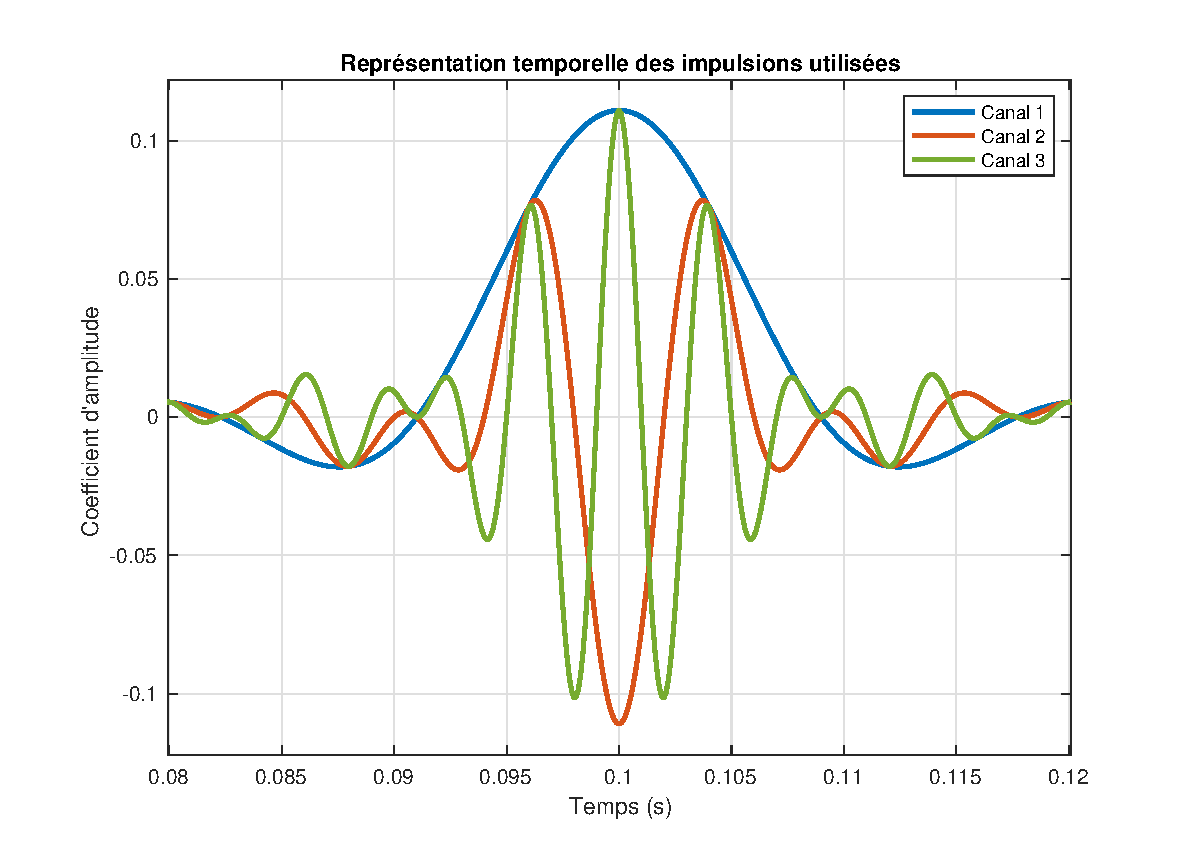
\includegraphics[height=0.4\textheight]{eps/impulse.eps}
	\caption{Représentation temporelle des impulsions utilisées pour multiplexer en 3 canaux.
			 Chaque des impulsions est sa réponse en bande de base modulée par sa porteuse.
			 Il est intéressant de constater que l'impulsion du canal 2 est inversée en
			 amplitude.}
	\label{fig:impulse}
\end{figure}

Les signaux modulés, leur puissance est normalisée à une quantité de milliwatt par seconde en divisant/multipliant les amplitudes par le facteur adéquat.
La puissance de chaque canal est évaluée en intégrant la norme au carré sur l'impédance caractéristique du milieu de propagation.

\begin{equation}
	P[s] = \frac{\frac{1}{N} \sum_{n = 0}^{N} s[n]^2}{Z_0}
\end{equation}

Le script \texttt{sender.m} affiche un récapitulatif de la transmission en temporel et fréquentiel avant de sommer tous les canaux pour les envoyer sur le seul lien physique disponible, le cable ou le rayonnement électro-magnétique.
Un exemple de ce récapitulatif est présenté à la figure~\ref{fig:sender}.

\begin{figure}[htbp]
	\centering
	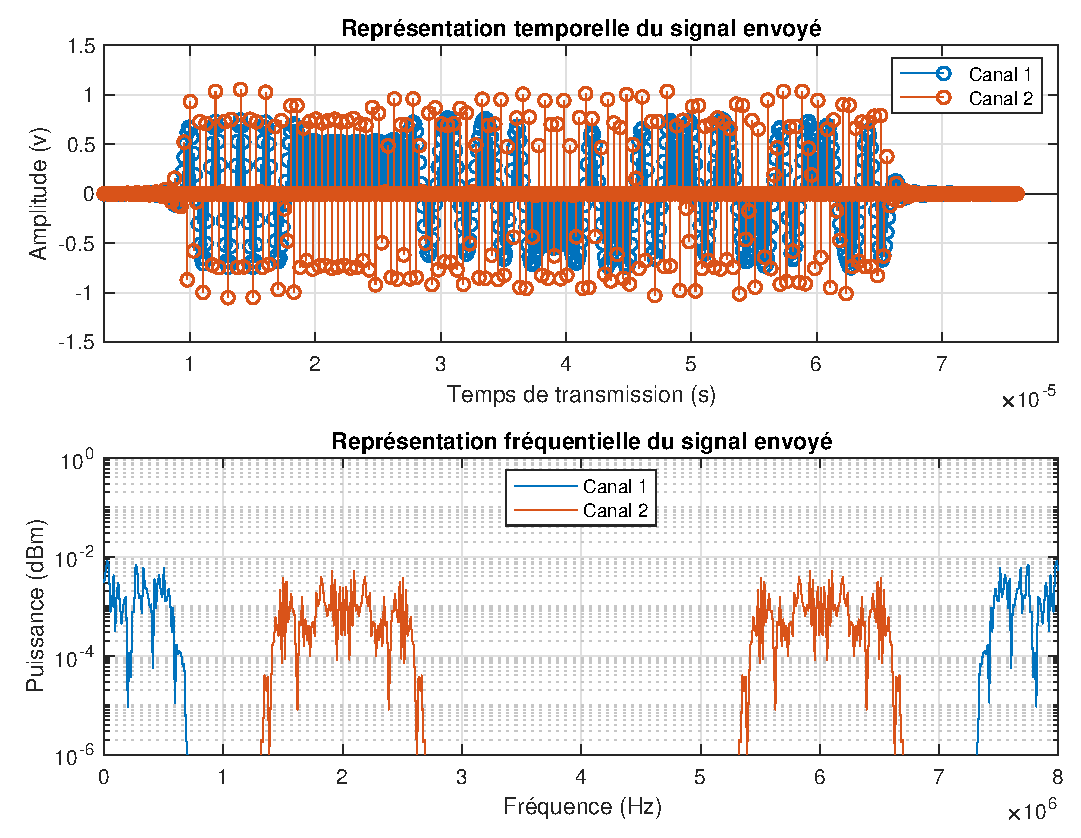
\includegraphics[height=0.45\textheight]{eps/sender.eps}
	\caption{Signaux de 50 bits chacun envoyés sur 2 canaux fréquentiels au rythme de 10 bit/s
			 avec une fréquence d'échantillonage de \SI{80}{\hertz}.}
	\label{fig:sender}
\end{figure}

\subsection{Canal}
Le fichier \texttt{canal.m} consultable à l'annexe~\ref{app:channel} à pour mission de simuler les effets du canal de communication.
Nous nous attendons à ce qu'il se comporte comme un filtre passe-bas, c.-à-d. une atténuation des amplitudes et un décalage temporelle.
Tout cela accompagné de bruit parasite.

Nous nous attendons à ce que le bruit sois de type AWGN, Additive white Gaussian noise, pouvant être symbolisé par une variable aléatoire de distribution normale et de moyenne nulle $g[k]\sim\mathcal{N}(0,\sigma^2)$.
Tout commence par la génération d'un vecteur aléatoire de distribution normale de même taille que le vecteur de donnée.
Ce vecteur aléatoire est ensuite filtré pour ne pas contenir de fréquence supérieure à celle de Nyquist.
L'intensité du bruit se règle en multipliant le vecteur obtenu, qui est de variance 1, par l'écart-type de la variance désiré.
Un facteur d'atténuation A borné tel que $\num{0.6} \leq A \leq \num{0.9}$ est également généré.
Le script effectue ensuite $S_2[k] = A \cdot S_1[k] + g[k]$ pour appliquer l'atténuation et le bruit.
Du \og{}zero-padding\fg{} est ajouté au début du signal pour simuler un décalage temporel.

\subsection{Receveur}
Le fichier \texttt{receiver.m} consultable à l'annexe~\ref{app:receiver} se charge de ramener les signaux transmis en bande de base et prend des décisions sur les valeurs mesurées à tous les $T_b$ instants en espérant retrouver le signal original.

Le script commence par générer des filtres de type Butterworth qui vont lui permettre de séparer les canaux.
Pour filtrer, on commence par obtenir la fraction polynomiale représentant le filtre analogique.
De cette fonction, on calcule la réponse fréquentiel entre la fréquence 0 et la fréquence d'échantillonnage.
On applique la transformé de Fourier inverse à cette réponse fréquentiel, et nous obtenons la réponse impulsionnelle du filtre.
Il suffit dès lors de convoluer les échantillons temporels de notre signal avec les réponses impulsionnelles calculées et nous séparons ainsi les bandes spectrales.
Nous calculons des filtres d'ordre 10, la figure~\ref{fig:filters} et ~\ref{fig:grpdelay} présentent les filtres permettant des séparer les deux canaux utilisé dans cette simulation.

Une fois les canaux séparés, il faut les ramener en bande de base.
On ne peut pas simplement diviser les signaux pas un cosinus de même fréquence que la porteuse car le déphasage entre les deux laisserait une composante sinusoïdale parasite dans nos échantillons démodulés.
Pour obtenir notre signal en bande de base, nous multiplions encore le signal modulé avec un cosinus à même fréquence, multiplier deux cosinus amène à additionner leur fréquence.
Nous filtrons ensuite ce signal doublement multiplié par un filtre passe-bas pour supprimer les porteuses envoyée dans de plus haute fréquence, et les fréquences restantes sont notre signal en bande de base.
En procédant de cette manière, nous contournons le problème d'estimation de la phase de la porteuse.

\begin{figure}[htbp]
	\centering
	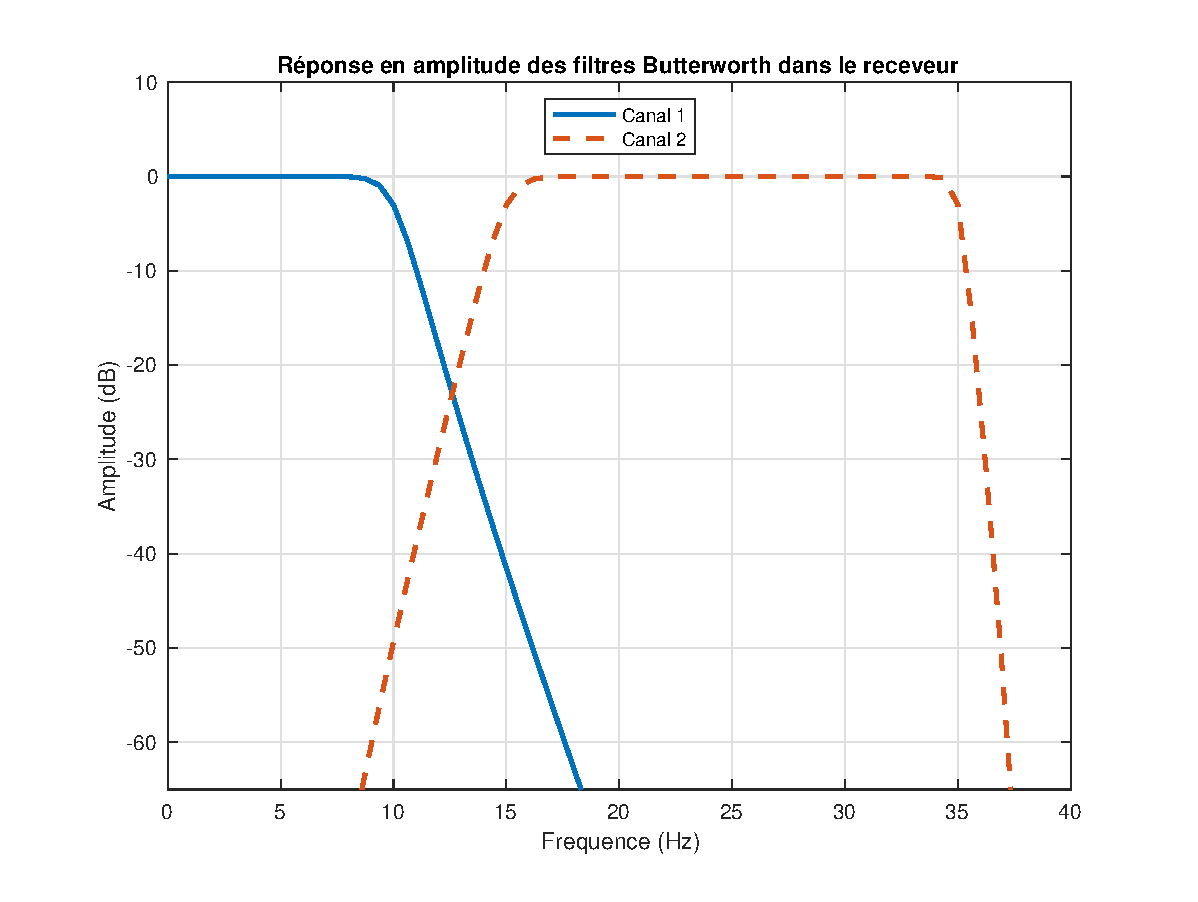
\includegraphics[height=0.4\textheight]{eps/filters.eps}
	\caption{Réponse en amplitude des filtres de type Butterworth utilisés dans le receveur
			 pour séparer les canaux.}
	\label{fig:filters}
\end{figure}

\begin{figure}[htbp]
	\centering
	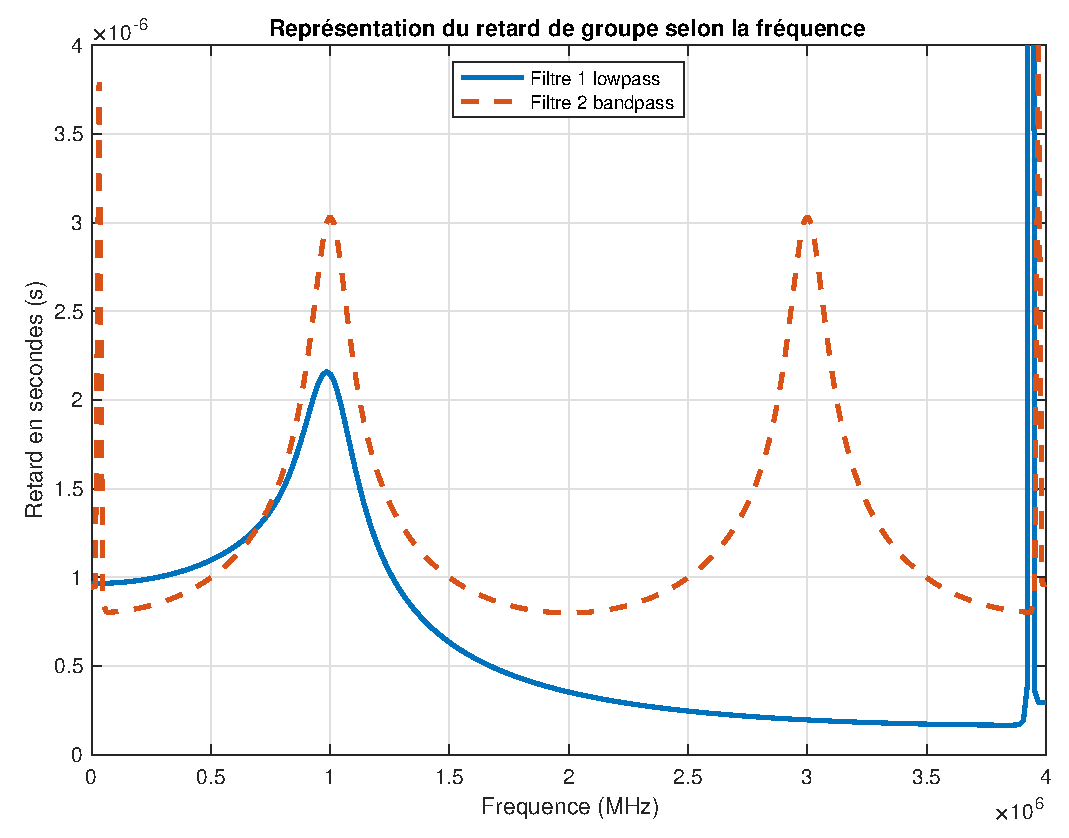
\includegraphics[height=0.45\textheight]{eps/grpdelay.eps}
	\caption{Retard de groupe des filtres de type Butterworth utilisés dans le receveur
			 pour séparer les canaux.
			 Le filtre 1 est un lowpass avec une fréquence de coupure à \SI{10}{\hertz}.
			 Le filtre 2 est un bandpass avec une fréquence de coupure basse à
			 \SI{25}{\hertz} et fréquence de coupure haute à \SI{35}{\hertz}.}
	\label{fig:grpdelay}
\end{figure}

Le script receveur affiche un récapitulatif de la transmission reçue, comme l'émetteur affiche une récapitulatif de la transmission envoyée.
Ces récapitulatifs permettent de comparer les signaux émis avant d'être sommé dans l'environnement de transmission, \textit{e.g.} un câble, et les signaux reçus après les avoir séparés par filtrage.
La figure~\ref{fig:receiver} du receveur doit être comparé avec la figure~\ref{fig:sender} de l'émetteur.
On peut constater que : temporellement le receveur a un message décalé de quelques échantillons ; et fréquentiellement un signal atténué de quelques dBm.

\begin{figure}[htbp]
	\centering
	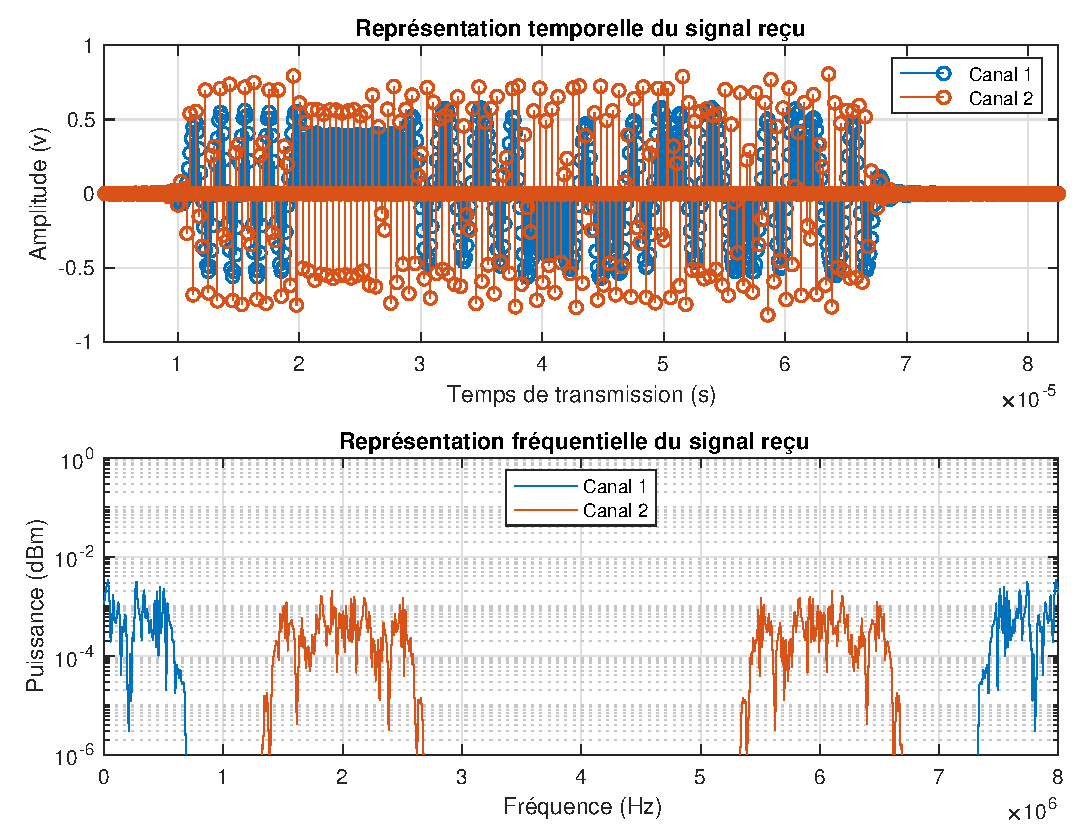
\includegraphics[height=0.45\textheight]{eps/receiver.eps}
	\caption{Signaux de 50 bits chacun envoyés sur 2 canaux fréquentiels au rythme de 10 bit/s
			 avec une fréquence d'échantillonage de \SI{80}{\hertz}.}
	\label{fig:receiver}
\end{figure}

Une fois le signal en bande de base recomposé, le recevoir doit repérer début du signal et capturer un échantillon tous les $T_b$ instant.
Depuis cet échantillon capturé, il doit prendre la décision de choisir si le code transmis était $+1$ ou $-1$.
La figure~\ref{fig:decimate} présente un exemple de capture d'échantillons effectuée par le receveur.

\begin{figure}[htbp]
	\centering
	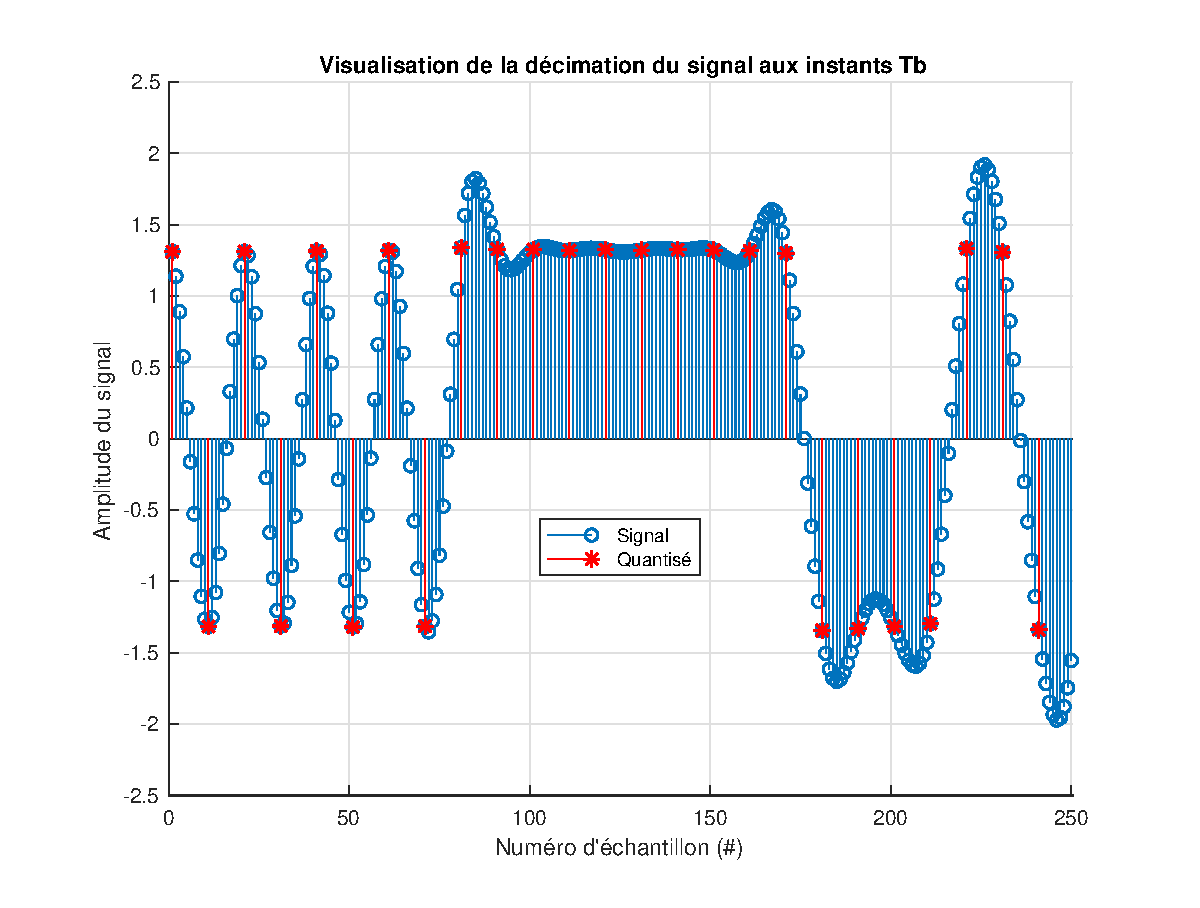
\includegraphics[height=0.45\textheight]{eps/decimate.eps}
	\caption{Visualisation de la capture d'échantillons pour le décideur.}
	\label{fig:decimate}
\end{figure}


%%%%%%%%%%%%%%%%%%%%%%
\section{Performances}


%%%%%%%%%%%%%%%%%%%%
\section{Conclusion}

\appendix
\clearpage

\section{Fichiers sources}
\label{sec:fichiers-sources}

\subsection{main.m}
\inputminted{matlab}{../main.m}
\label{app:main}

\subsection{parameters.m}
\inputminted{matlab}{../parameters.m}
\label{app:paremeters}

\subsection{sender.m}
\inputminted{matlab}{../sender.m}
\label{app:sender}

\subsection{channel.m}
\inputminted{matlab}{../channel.m}
\label{app:channel}

\subsection{receiver.m}
\inputminted{matlab}{../receiver.m}
\label{app:receiver}

\end{document}
